\documentclass[../report.tex]{subfiles}

\begin{document}
\subsection{Bài toán} 
Mô phỏng sự di chuyển của các xe trên các đường và tại các ngã tư. 
Từ đó có thể tính các thông số trong quá trình di chuyển như quãng đường đi được, 
thời gian đi, lượng năng lượng tiêu thụ, ... của mỗi xe. 
Các xe di chuyển dựa trên hướng đi được xác định sẵn. 
\begin{figure}[H]
\centering
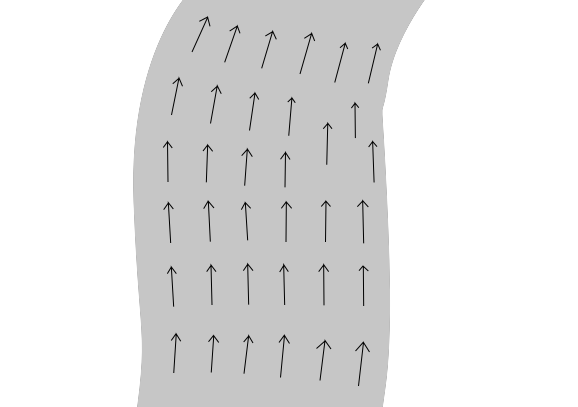
\includegraphics[width=10cm]{figures/normal-road.png}
\caption{Trường vector chỉ định hướng đi trên một đoạn đường}
\end{figure}

Các tác tử được được chia thành hai loại: 
\begin{itemize}
\item Tác tử tĩnh: Đại diện cho đường đi. 
\item Tác tử động: Đại diện cho các xe và các điểm sinh ra các xe. 
\end{itemize}

Đường đi được chia làm hai loại: 
\begin{itemize}
\item Đường đi một chiều
\item Ngã rẽ. 
\end{itemize}

\begin{figure}[H]
\centering

\includegraphics[width=8cm]{figures/cross-road.png}
\caption{Màu xanh: Đường đi bình thường - Màu đỏ: Ngã rẽ}
\end{figure}

\subsection{Tác tử tĩnh - đường đi}
Các đường đi được xây dựng bởi các cell, mỗi cell là một object thuộc một trong 2 kiểu: 
\begin{itemize}
\item \textbf{NormalRoad}: Chứa thông tin về hướng di chuyển của các xe 
    trên đường một chiều, chứa cạnh tương ứng trên đồ thị đường đi. 
\item \textbf{TurningRoad}: Chứa thông tin về hướng di chuyển của các xe tương ứng từ cạnh này sang cạnh kia của đồ thị đường đi. 
\end{itemize}

\begin{figure}[H]
\centering
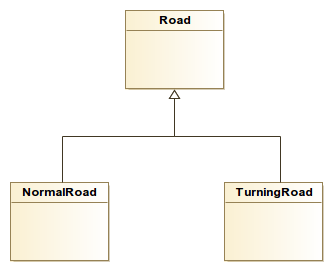
\includegraphics[width=6cm]{figures/road-diagram.png}
\caption{Biểu đồ lớp}
\end{figure}

\subsection{Tác tử động}
\begin{itemize}
\item Các xe - \textbf{Car}: Mỗi xe chứa thông tin về vận tốc, năng lượng tiêu thụ. 
Ở mỗi bước thời gian của mô phỏng, xe xác định hướng dựa trên 
đường đi mà nó đang đứng (nếu đang ở đường đi một chiều - \textbf{NormalRoad}) 
hoặc dựa vào cặp cạnh (chọn ngẫu nhiên) trên đồ thị đường đi để xác định hướng 
đi dựa trên ngã rẽ mà nó đang đứng (nếu đang ở đoạn ngã rẽ - \textbf{TurningRoad}).  \\
Từ vận tốc và hướng đi xác định được vị trí ở bước thời gian tiếp theo. 
Các xe có thể quan sát vị trí các xe xung quanh để quyết định có nên giảm tốc độ / tăng tốc độ hay không. 
\item Các điểm sinh xe - \textbf{CarGenerator}: Có tọa độ là một ví trí nào đó trên các đường một chiều, 
tọa độ của các xe được sinh ngẫu nhiên xung quanh điểm đó. 
\end{itemize}

\subsection{Kết quả đạt được}
\begin{figure}[H]
\centering
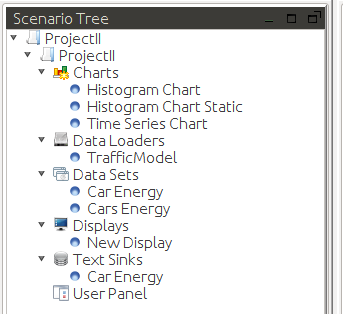
\includegraphics[width=6cm]{figures/tree.png}
\caption{Thiết lập được sử dụng}
\end{figure}

\begin{figure}[H]
\centering
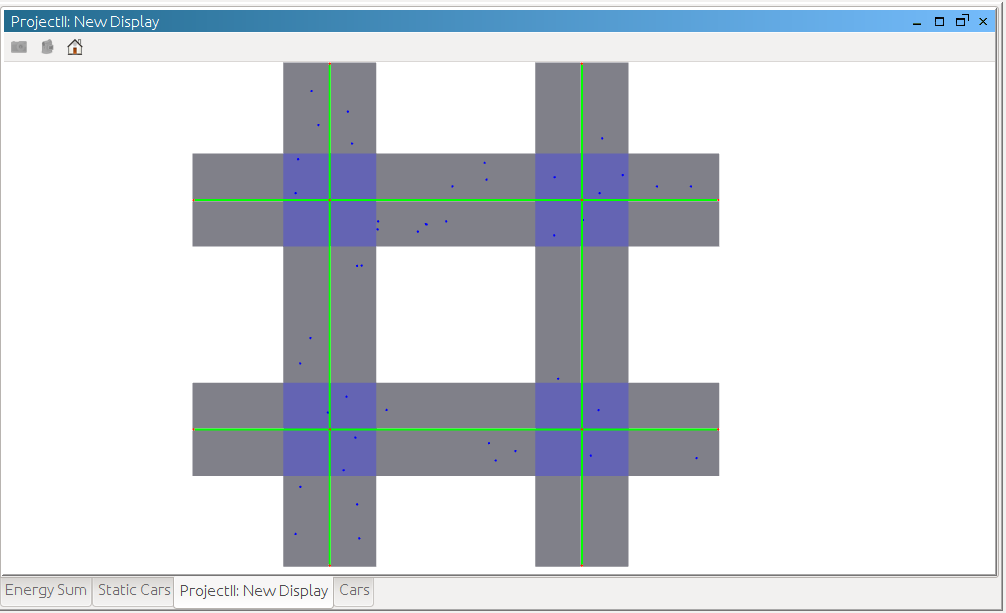
\includegraphics[width=\textwidth]{figures/render.png}
\caption{Mô phỏng được hiển thị}
\end{figure}

\begin{figure}[H]
\centering
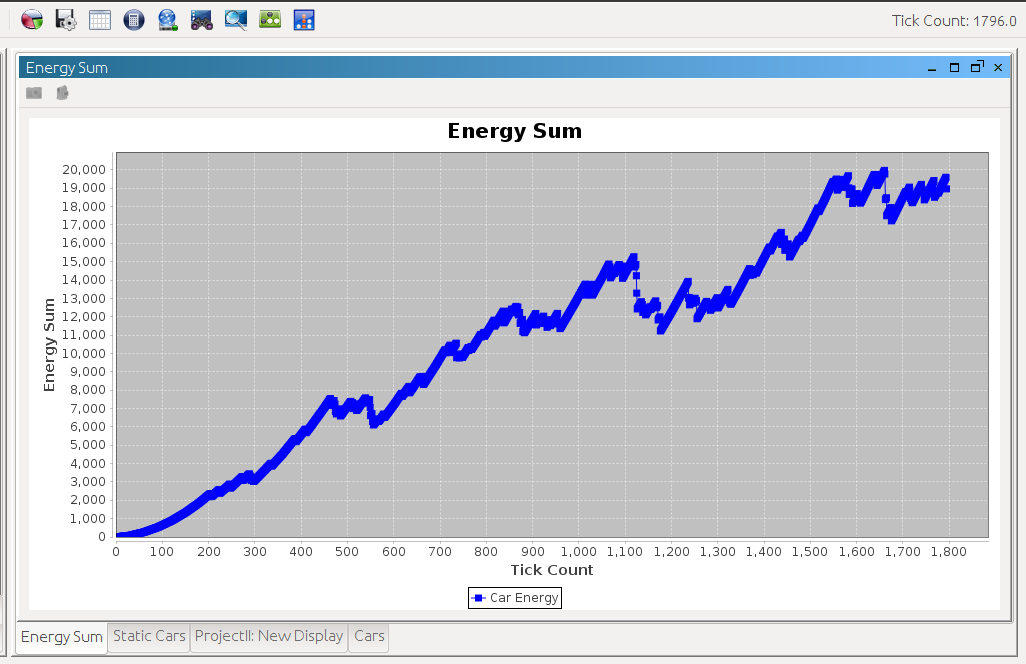
\includegraphics[width=14cm]{figures/time-series.png}
\caption{Biểu đồ tổng năng lượng tiêu thụ theo thời gian}
\end{figure}

\begin{figure}[H]
\centering
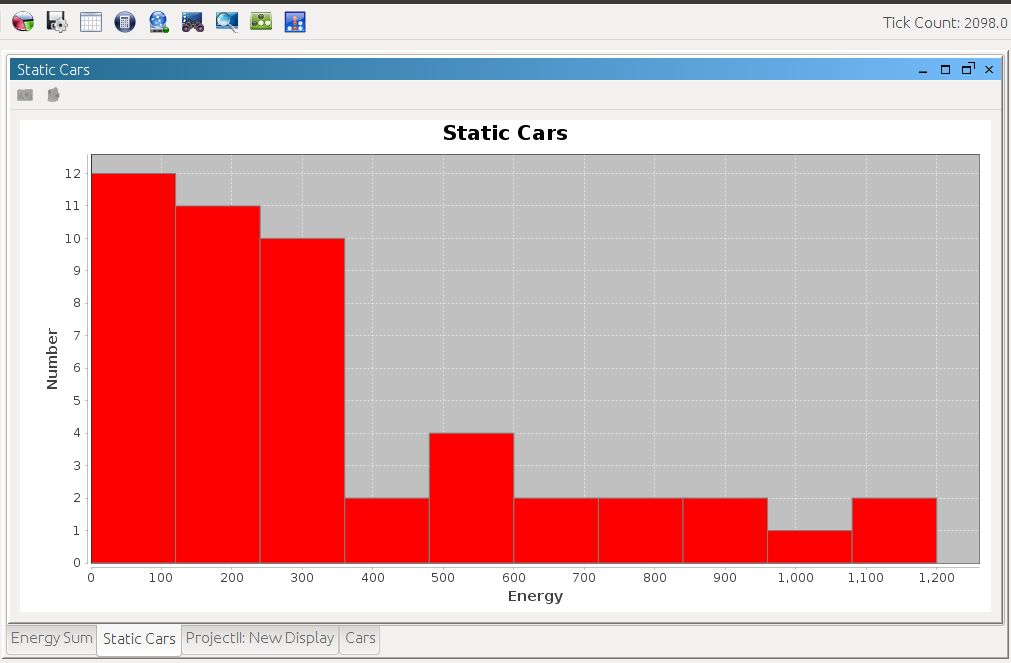
\includegraphics[width=14cm]{figures/static-histogram.png}
\caption{Biểu đồ histogram năng lượng tiêu thụ với biên cố định}
\end{figure}

\begin{figure}[H]
\centering
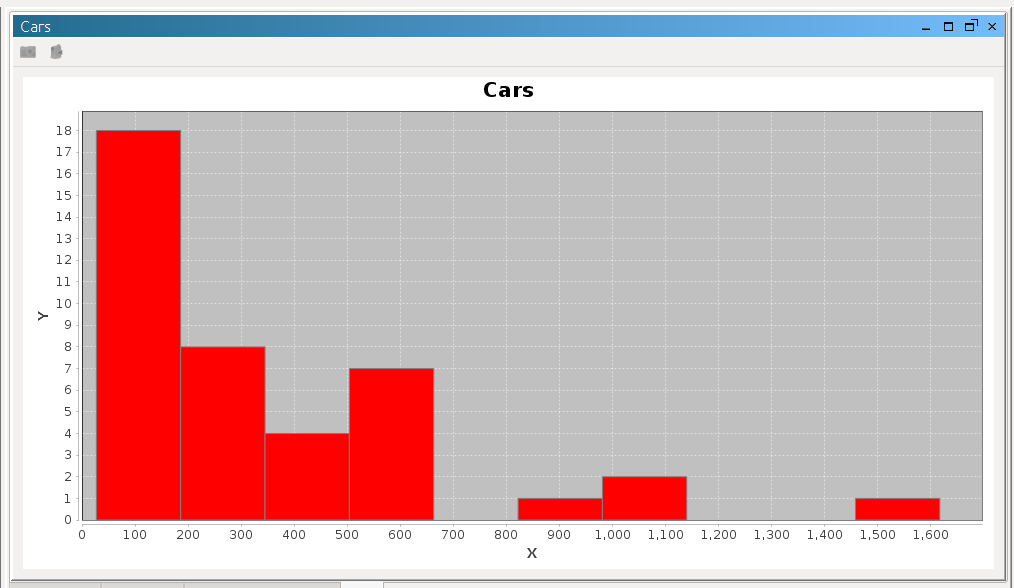
\includegraphics[width=14cm]{figures/dynamic-histogram.png}
\caption{Biểu đồ histogram năng lượng tiêu thụ với biên thay đổi}
\end{figure}

\begin{figure}[H]
\centering
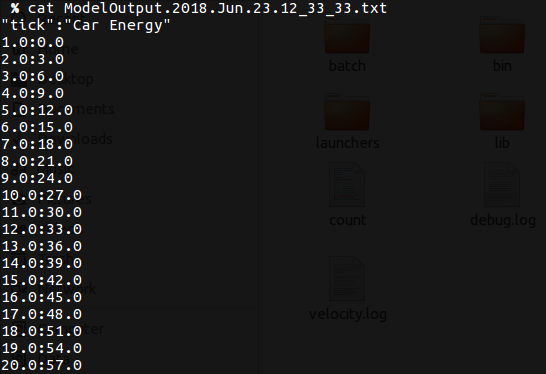
\includegraphics[width=10cm]{figures/output-file.png}
\caption{File chứa tổng năng lượng tiêu thụ ở mỗi bước thời gian}
\end{figure}

\end{document}
